
\item A round cone with half-angle \( \alpha = 30^\circ \) and the radius of the base \( R = 5.0 \) cm rolls uniformly and without slipping over a horizontal plane as shown in Fig. 1.8. The cone apex is hinged at the point \( O \) which is on the same level with the point \( C \), the cone base centre. The velocity of point \( C \) is \( v = 10.0 \) cm/s. Find the moduli of
\begin{center}
    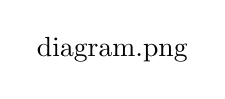
\begin{tikzpicture}
        \node at (0, 0) {diagram.png};
    \end{tikzpicture}
\end{center}
\begin{enumerate}
    \item the vector of the angular velocity of the cone and the angle it forms with the vertical;
    \item the vector of the angular acceleration of the cone.
\end{enumerate}

\begin{solution}
    \begin{center}
        \begin{tikzpicture}
            \pic at (0, 0) {frame=3cm};
        \end{tikzpicture}
    \end{center}
    
    \begin{align*}
        \intertext{(a) Let the axis of the cone ($OC$) rotate in anticlockwise sense with constant angular velocity $\omega'$ and the cone itself about its own axis ($OC$) in clockwise sense with angular velocity $\omega_0$. Then the resultant angular velocity of the cone}
        \omega &= \omega' + \omega_0\\
        \intertext{As the rolling is pure the magnitudes of the vectors $\omega'$ and $\omega_0$ can be easily found from the figure as}
        \omega' &= \dfrac{v}{R \cot \alpha} \quad \text{and} \quad \omega_0 = \dfrac{v}{R}\\
        \intertext{As $\omega \perp \omega_0$, hence}
        \omega &= \sqrt{\omega'^2 + \omega_0^2}\\
        &= \sqrt{\left(\dfrac{v}{R \cot \alpha}\right)^2 + \left(\dfrac{v}{R}\right)^2}\\
        &= \dfrac{v}{R \cos \alpha} = 2.32 \text{ rad/s}
        \intertext{(b) Vector of angular acceleration}
        \beta &= \dfrac{d \omega}{dt} = \dfrac{d (\omega' + \omega_0)}{dt} = \dfrac{d \omega_0}{dt} \quad \text{(as \(\omega'\) = constant)}\\
        \intertext{If any vector $\mathbf{a}$ (say) rotates with angular velocity $\omega$ keeping its values constant then $d\mathbf{a}/dt = \omega \times \mathbf{a}$. The vector $\omega_0$ keeping its magnitude constant rotates about the $OO'$ axis with the angular velocity $\omega'$. So $d\omega_0/dt = (\omega' \times \omega_0)$. Hence}
        \beta &= \omega' \times \omega_0 \quad \text{The magnitude of the vector $\beta$ is equal to $\beta = \omega' \omega_0$ (as $\omega' \perp \omega_0$).}\\
        \intertext{So,}
        \beta &= \dfrac{v}{R \cot \alpha} \left( \dfrac{v}{R} \right)\\
        &= \dfrac{v^2}{R^2} \tan \alpha = 2.3 \text{ rad/s}^2, \text{ on putting the values of } v, R \text{ and } \alpha
        \intertext{Alternate:}
        \intertext{Vector $\omega_0$ is turning keeping the magnitude constant. To find $d\omega_0$, let us make a vector diagram as shown in the figure. The circle shown in the figure has the radius $\omega_0$ and the tail of $\omega_0$ and of $\omega_0 + d\omega_0$ coincides at the center of the circle.}
        \intertext{Let $\omega_0$ turn by the small angle $d\phi$ in the differential time interval $dt$, so $d\phi = \omega' dt$. Thus $|d\omega_0| \approx \text{arc length} = \omega_0 d\phi = \omega_0 \omega' dt$. As $\omega_0$ is along radial line and $d\omega_0$ is along the tangent in the turning sense of $\omega_0$ so $d\omega_0 \perp \omega_0$. In vector form}
        d\omega_0 &= (\omega' \times \omega_0) dt\\
        \intertext{Hence,}
        \beta &= \dfrac{d\omega_0}{dt} = (\omega' \times \omega_0)
    \end{align*}
\end{solution}
